% Created by tikzDevice version 0.12.6 on 2024-06-02 21:53:07
% !TEX encoding = UTF-8 Unicode
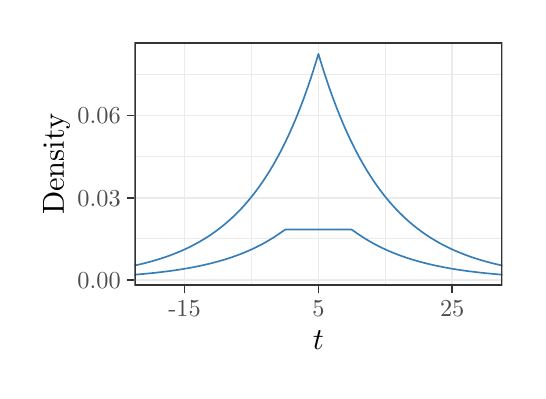
\begin{tikzpicture}[x=1pt,y=1pt]
\definecolor{fillColor}{RGB}{255,255,255}
\path[use as bounding box,fill=fillColor,fill opacity=0.00] (0,0) rectangle (177.06,123.94);
\begin{scope}
\path[clip] (  0.00,  0.00) rectangle (177.06,123.94);
\definecolor{drawColor}{RGB}{255,255,255}
\definecolor{fillColor}{RGB}{255,255,255}

\path[draw=drawColor,line width= 0.6pt,line join=round,line cap=round,fill=fillColor] ( -0.00,  0.00) rectangle (177.06,123.94);
\end{scope}
\begin{scope}
\path[clip] ( 38.56, 30.69) rectangle (171.56,118.44);
\definecolor{fillColor}{RGB}{255,255,255}

\path[fill=fillColor] ( 38.56, 30.69) rectangle (171.56,118.44);
\definecolor{drawColor}{gray}{0.92}

\path[draw=drawColor,line width= 0.3pt,line join=round] ( 38.56, 47.62) --
	(171.56, 47.62);

\path[draw=drawColor,line width= 0.3pt,line join=round] ( 38.56, 77.35) --
	(171.56, 77.35);

\path[draw=drawColor,line width= 0.3pt,line join=round] ( 38.56,107.08) --
	(171.56,107.08);

\path[draw=drawColor,line width= 0.3pt,line join=round] ( 80.88, 30.69) --
	( 80.88,118.44);

\path[draw=drawColor,line width= 0.3pt,line join=round] (129.24, 30.69) --
	(129.24,118.44);

\path[draw=drawColor,line width= 0.6pt,line join=round] ( 38.56, 32.75) --
	(171.56, 32.75);

\path[draw=drawColor,line width= 0.6pt,line join=round] ( 38.56, 62.49) --
	(171.56, 62.49);

\path[draw=drawColor,line width= 0.6pt,line join=round] ( 38.56, 92.22) --
	(171.56, 92.22);

\path[draw=drawColor,line width= 0.6pt,line join=round] ( 56.69, 30.69) --
	( 56.69,118.44);

\path[draw=drawColor,line width= 0.6pt,line join=round] (105.06, 30.69) --
	(105.06,118.44);

\path[draw=drawColor,line width= 0.6pt,line join=round] (153.42, 30.69) --
	(153.42,118.44);
\definecolor{drawColor}{RGB}{55,126,184}

\path[draw=drawColor,line width= 0.6pt,line join=round] ( 38.56, 34.67) --
	( 39.89, 34.78) --
	( 41.22, 34.90) --
	( 42.55, 35.02) --
	( 43.88, 35.15) --
	( 45.21, 35.28) --
	( 46.54, 35.43) --
	( 47.87, 35.58) --
	( 49.20, 35.74) --
	( 50.53, 35.91) --
	( 51.86, 36.08) --
	( 53.19, 36.27) --
	( 54.52, 36.47) --
	( 55.85, 36.68) --
	( 57.18, 36.90) --
	( 58.51, 37.14) --
	( 59.84, 37.39) --
	( 61.17, 37.65) --
	( 62.50, 37.92) --
	( 63.83, 38.22) --
	( 65.16, 38.53) --
	( 66.49, 38.85) --
	( 67.82, 39.20) --
	( 69.15, 39.56) --
	( 70.48, 39.95) --
	( 71.81, 40.35) --
	( 73.14, 40.78) --
	( 74.47, 41.24) --
	( 75.80, 41.72) --
	( 77.13, 42.22) --
	( 78.46, 42.76) --
	( 79.79, 43.32) --
	( 81.12, 43.92) --
	( 82.45, 44.55) --
	( 83.78, 45.22) --
	( 85.11, 45.92) --
	( 86.44, 46.67) --
	( 87.77, 47.46) --
	( 89.10, 48.29) --
	( 90.43, 49.17) --
	( 91.76, 50.09) --
	( 93.09, 50.98) --
	( 94.42, 50.98) --
	( 95.75, 50.98) --
	( 97.08, 50.98) --
	( 98.41, 50.98) --
	( 99.74, 50.98) --
	(101.07, 50.98) --
	(102.40, 50.98) --
	(103.73, 50.98) --
	(105.06, 50.98) --
	(106.39, 50.98) --
	(107.72, 50.98) --
	(109.05, 50.98) --
	(110.38, 50.98) --
	(111.71, 50.98) --
	(113.04, 50.98) --
	(114.37, 50.98) --
	(115.70, 50.98) --
	(117.03, 50.98) --
	(118.36, 50.09) --
	(119.69, 49.17) --
	(121.02, 48.29) --
	(122.35, 47.46) --
	(123.68, 46.67) --
	(125.01, 45.92) --
	(126.34, 45.22) --
	(127.67, 44.55) --
	(129.00, 43.92) --
	(130.33, 43.32) --
	(131.66, 42.76) --
	(132.99, 42.22) --
	(134.32, 41.72) --
	(135.65, 41.24) --
	(136.98, 40.78) --
	(138.31, 40.35) --
	(139.64, 39.95) --
	(140.97, 39.56) --
	(142.30, 39.20) --
	(143.63, 38.85) --
	(144.96, 38.53) --
	(146.29, 38.22) --
	(147.62, 37.92) --
	(148.95, 37.65) --
	(150.28, 37.39) --
	(151.61, 37.14) --
	(152.94, 36.90) --
	(154.27, 36.68) --
	(155.60, 36.47) --
	(156.93, 36.27) --
	(158.26, 36.08) --
	(159.59, 35.91) --
	(160.92, 35.74) --
	(162.25, 35.58) --
	(163.58, 35.43) --
	(164.91, 35.28) --
	(166.24, 35.15) --
	(167.57, 35.02) --
	(168.90, 34.90) --
	(170.23, 34.78) --
	(171.56, 34.67);

\path[draw=drawColor,line width= 0.6pt,line join=round] ( 38.56, 37.98) --
	( 39.89, 38.27) --
	( 41.22, 38.58) --
	( 42.55, 38.91) --
	( 43.88, 39.26) --
	( 45.21, 39.63) --
	( 46.54, 40.02) --
	( 47.87, 40.43) --
	( 49.20, 40.86) --
	( 50.53, 41.32) --
	( 51.86, 41.81) --
	( 53.19, 42.32) --
	( 54.52, 42.86) --
	( 55.85, 43.43) --
	( 57.18, 44.03) --
	( 58.51, 44.67) --
	( 59.84, 45.35) --
	( 61.17, 46.06) --
	( 62.50, 46.81) --
	( 63.83, 47.60) --
	( 65.16, 48.44) --
	( 66.49, 49.33) --
	( 67.82, 50.27) --
	( 69.15, 51.26) --
	( 70.48, 52.31) --
	( 71.81, 53.41) --
	( 73.14, 54.58) --
	( 74.47, 55.81) --
	( 75.80, 57.12) --
	( 77.13, 58.49) --
	( 78.46, 59.95) --
	( 79.79, 61.49) --
	( 81.12, 63.11) --
	( 82.45, 64.83) --
	( 83.78, 66.64) --
	( 85.11, 68.56) --
	( 86.44, 70.58) --
	( 87.77, 72.72) --
	( 89.10, 74.98) --
	( 90.43, 77.37) --
	( 91.76, 79.89) --
	( 93.09, 82.56) --
	( 94.42, 85.37) --
	( 95.75, 88.35) --
	( 97.08, 91.49) --
	( 98.41, 94.81) --
	( 99.74, 98.32) --
	(101.07,102.03) --
	(102.40,105.94) --
	(103.73,110.08) --
	(105.06,114.45) --
	(106.39,110.08) --
	(107.72,105.94) --
	(109.05,102.03) --
	(110.38, 98.32) --
	(111.71, 94.81) --
	(113.04, 91.49) --
	(114.37, 88.35) --
	(115.70, 85.37) --
	(117.03, 82.56) --
	(118.36, 79.89) --
	(119.69, 77.37) --
	(121.02, 74.98) --
	(122.35, 72.72) --
	(123.68, 70.58) --
	(125.01, 68.56) --
	(126.34, 66.64) --
	(127.67, 64.83) --
	(129.00, 63.11) --
	(130.33, 61.49) --
	(131.66, 59.95) --
	(132.99, 58.49) --
	(134.32, 57.12) --
	(135.65, 55.81) --
	(136.98, 54.58) --
	(138.31, 53.41) --
	(139.64, 52.31) --
	(140.97, 51.26) --
	(142.30, 50.27) --
	(143.63, 49.33) --
	(144.96, 48.44) --
	(146.29, 47.60) --
	(147.62, 46.81) --
	(148.95, 46.06) --
	(150.28, 45.35) --
	(151.61, 44.67) --
	(152.94, 44.03) --
	(154.27, 43.43) --
	(155.60, 42.86) --
	(156.93, 42.32) --
	(158.26, 41.81) --
	(159.59, 41.32) --
	(160.92, 40.86) --
	(162.25, 40.43) --
	(163.58, 40.02) --
	(164.91, 39.63) --
	(166.24, 39.26) --
	(167.57, 38.91) --
	(168.90, 38.58) --
	(170.23, 38.27) --
	(171.56, 37.98);
\definecolor{drawColor}{gray}{0.20}

\path[draw=drawColor,line width= 0.9pt,line join=round,line cap=round] ( 38.56, 30.69) rectangle (171.56,118.44);
\end{scope}
\begin{scope}
\path[clip] (  0.00,  0.00) rectangle (177.06,123.94);
\definecolor{drawColor}{gray}{0.30}

\node[text=drawColor,anchor=base east,inner sep=0pt, outer sep=0pt, scale=  0.88] at ( 33.61, 29.72) {0.00};

\node[text=drawColor,anchor=base east,inner sep=0pt, outer sep=0pt, scale=  0.88] at ( 33.61, 59.46) {0.03};

\node[text=drawColor,anchor=base east,inner sep=0pt, outer sep=0pt, scale=  0.88] at ( 33.61, 89.19) {0.06};
\end{scope}
\begin{scope}
\path[clip] (  0.00,  0.00) rectangle (177.06,123.94);
\definecolor{drawColor}{gray}{0.20}

\path[draw=drawColor,line width= 0.6pt,line join=round] ( 35.81, 32.75) --
	( 38.56, 32.75);

\path[draw=drawColor,line width= 0.6pt,line join=round] ( 35.81, 62.49) --
	( 38.56, 62.49);

\path[draw=drawColor,line width= 0.6pt,line join=round] ( 35.81, 92.22) --
	( 38.56, 92.22);
\end{scope}
\begin{scope}
\path[clip] (  0.00,  0.00) rectangle (177.06,123.94);
\definecolor{drawColor}{gray}{0.20}

\path[draw=drawColor,line width= 0.6pt,line join=round] ( 56.69, 27.94) --
	( 56.69, 30.69);

\path[draw=drawColor,line width= 0.6pt,line join=round] (105.06, 27.94) --
	(105.06, 30.69);

\path[draw=drawColor,line width= 0.6pt,line join=round] (153.42, 27.94) --
	(153.42, 30.69);
\end{scope}
\begin{scope}
\path[clip] (  0.00,  0.00) rectangle (177.06,123.94);
\definecolor{drawColor}{gray}{0.30}

\node[text=drawColor,anchor=base,inner sep=0pt, outer sep=0pt, scale=  0.88] at ( 56.69, 19.68) {-15};

\node[text=drawColor,anchor=base,inner sep=0pt, outer sep=0pt, scale=  0.88] at (105.06, 19.68) {5};

\node[text=drawColor,anchor=base,inner sep=0pt, outer sep=0pt, scale=  0.88] at (153.42, 19.68) {25};
\end{scope}
\begin{scope}
\path[clip] (  0.00,  0.00) rectangle (177.06,123.94);
\definecolor{drawColor}{RGB}{0,0,0}

\node[text=drawColor,anchor=base,inner sep=0pt, outer sep=0pt, scale=  1.10] at (105.06,  7.64) {$t$};
\end{scope}
\begin{scope}
\path[clip] (  0.00,  0.00) rectangle (177.06,123.94);
\definecolor{drawColor}{RGB}{0,0,0}

\node[text=drawColor,rotate= 90.00,anchor=base,inner sep=0pt, outer sep=0pt, scale=  1.10] at ( 13.08, 74.56) {Density};
\end{scope}
\end{tikzpicture}
